

\section{ASLR}
\begin{frame}{address space layout randomization (ASLR)}
    \begin{itemize}
    \item vary the location of things in memory
    \item including the stack
    \item designed to make exploiting memory errors harder
    \item will talk more about later
    \end{itemize}
\end{frame}


\subsection{what it is}

\begin{frame}{address space layout randomization (ASLR)}
    \begin{itemize}
    \item assume: addresses don't leak
    \item choose \myemph{random} addresses each time
        \begin{itemize}
        \item for \myemph{everything}, not just the stack
        \end{itemize}
    \item \myemph{enough possibilities} that attacker won't ``get lucky''
    \item should prevent exploits --- can't write GOT/shellcode location
    \end{itemize}
\end{frame}

\begin{frame}[fragile]{recall: position independent executables}
\begin{Verbatim}
...
EXEC_P, D_PAGED
...
LOAD off    0x0000000 vaddr \myemph{0x400000} paddr 0x0400000 align 2**12
     filesz 0x00006c8 memsz 0x0006c8 flags r--
LOAD off    0x0001000 vaddr 0x401000 paddr 0x0401000 align 2**12
     filesz 0x01a7865 memsz 0x1a7865 flags r-x
\end{Verbatim}
    \begin{itemize}
    \item some executables had LOADs at fixed addresses
        \begin{itemize}
        \item machine code might use hard-coded addresses
        \end{itemize}
    \item can't randomize program addresses
    \item others did not (marked DYNAMIC)
    \end{itemize}
\begin{Verbatim}[fontsize=\fontsize{9}{10}\selectfont,commandchars=\\\{\}]
...
HAS_SYMS, \myemph{DYNAMIC}, D_PAGED
...
LOAD off    0x000000 vaddr \myemph{0x000000} paddr 0x000000 align 2**12
     filesz 0x0036f8 memsz 0x0036f8 flags r--
LOAD off    0x004000 vaddr 0x004000 paddr 0x004000 align 2**12
...
\end{Verbatim}
\end{frame}


\subsection{how much entropy}
\usetikzlibrary{calc,positioning,patterns,shapes.callouts}

\begin{frame}{Linux stack randomization (x86-64)}
\begin{itemize}
    \item 1. choose random number between \texttt{0} and \tikzmark{range}\myemph<2>{\texttt{0x3F FFFF}}
    \item 2. stack starts at \texttt{0x7FFF FFFF FFFF} - \textit{random number} $\times$ \texttt{0x1000}
        \begin{itemize}
        \item randomization disabled? \textit{random number} $= 0$
        \item times \texttt{0x1000} because OS has to allocate whole pages (0x1000 bytes)
        \end{itemize}
\end{itemize}
\begin{tikzpicture}[overlay,remember picture]
\node[my callout=range] at ([yshift=-1cm]current page.center) {
    16 GB range!
};
\end{tikzpicture}
\end{frame}


\begin{frame}<1>[fragile,label=aslr64]{program memory (x86-64 Linux; ASLR)}
\begin{tikzpicture}[remember picture]
\tikzset{
    mylabel/.style={font=\ttfamily,align=center,append after command={([xshift=.1cm]\tikzlastnode.west) edge[ultra thick] ++(-.2cm,0cm)}},
    mybox/.style={draw,rectangle,minimum width=7cm,fill=white},
    myhigh/.style={draw,rectangle,line width=1mm, draw=blue!80!black,opacity=.3},
}
\node[mybox,minimum height=.5cm,inner ysep=0mm,pattern=north west lines,pattern color=black!50!white] (kernel) {Used by OS};
\begin{pgfonlayer}{bg}
    \node[right=1mm of kernel.north east,mylabel] (topLabel) {0xFFFF FFFF FFFF FFFF};
    \node[right=1mm of kernel.south east,mylabel] {0xFFFF 8000 0000 0000};
\end{pgfonlayer}
\node[mybox, minimum height=.5cm, below=.45cm of kernel] (stack) {Stack};
\begin{pgfonlayer}{bg}
    \node[right=1mm of stack.north east,mylabel] {\myemph<1>{$\pm$ 0x004 0000 0000}};
\end{pgfonlayer}
\node[mybox, minimum height=.5cm, below=0.5cm of stack] (heapB) {mmap/non-fixed exe/libs};
\begin{pgfonlayer}{bg}
    \node[right=1mm of heapB.north east,mylabel] (heapBLabel) {\myemph<1>{$\pm$ 0x100 0000 0000}};
    \node[below=0mm of heapBLabel,font=\small,inner sep=0mm] {(filled from top with ASLR)};
\end{pgfonlayer}
%\begin{pgfonlayer}{bg}
%    \node[right=1mm of heapB.south east,mylabel] (heapBLabel) {0x0000 2baa aaaa b000 \\ $\pm$ 0x100 0000 0000\*};
%\end{pgfonlayer}
\node[mybox, minimum height=.5cm, below=0.5cm of heapB] (heap) {Heap (brk/sbrk)};
\begin{pgfonlayer}{bg}
\node[right=1mm of heap.south east,mylabel] (heapBLabel) {\myemph<1>{$\pm$ 0x200 0000}};
\end{pgfonlayer}
\node[mybox, minimum height=.5cm, below=0.2mm of heap] (data) {fixed exe writeable (sometimes)};
\begin{pgfonlayer}{bg}
\node[right=1mm of data.south east,mylabel] (bottomLabel) {\myemph<2-3>{0x0000 0000 0060 0000}*};
\node[below=0mm of bottomLabel,font=\small,inner sep=0mm] {(constants + 2MB alignment)};
\end{pgfonlayer}
\node[mybox, minimum height=.5cm, below=0.6cm of data] (sdata) {fixed exe code/data};
\begin{pgfonlayer}{bg}
\node[right=1mm of sdata.south east,mylabel] (sbottomLabel) {\myemph<2-3>{0x0000 0000 0040 0000}};
\end{pgfonlayer}
\coordinate (memBottom) at ($(sdata.south east) + (0mm, -2mm)$);
\begin{pgfonlayer}{bg}
\draw[pattern=north west lines, pattern color=black!40!white] (kernel.north west) rectangle (memBottom);
\end{pgfonlayer}

\begin{visibleenv}<3>
    \begin{scope}[overlay]
    \node[draw=red,ultra thick,fill=white,anchor=center,
          inner sep=.5cm,font=\Large] at (current page.center) {
        why are these addresses fixed?
    }; 
    \end{scope}
\end{visibleenv}

\end{tikzpicture}
\end{frame}

\begin{frame}{program memory (x86-32 Linux; ASLR)}
\begin{tikzpicture}
\tikzset{
    mylabel/.style={font=\ttfamily,align=center,append after command={([xshift=.1cm]\tikzlastnode.west) edge[ultra thick] ++(-.2cm,0cm)}},
    mybox/.style={draw,rectangle,minimum width=7cm,fill=white},
    myhigh/.style={draw,rectangle,line width=1mm, draw=blue!80!black,opacity=.3},
}
\node[mybox,minimum height=.5cm,inner ysep=0mm,pattern=north west lines,pattern color=black!50!white] (kernel) {Used by OS};
\begin{pgfonlayer}{bg}
    \node[right=1mm of kernel.north east,mylabel] (topLabel) {0xFFFF FFFF};
    \node[right=1mm of kernel.south east,mylabel] {0xC000 0000};
\end{pgfonlayer}
\node[mybox, minimum height=.5cm, below=.5cm of kernel] (stack) {Stack};
\begin{pgfonlayer}{bg}
    \node[right=1mm of stack.north east,mylabel] {\myemph{$\pm$ 0x080 0000} (default)};
\end{pgfonlayer}
\node[mybox, minimum height=.5cm, below=0.5cm of stack] (heapB) {Dynamic/Libraries (mmap)};
\begin{pgfonlayer}{bg}
    \node[right=1mm of heapB.north east,mylabel] (heapBLabel) {\myemph{$\pm$ 0x008 0000} (default)};
\end{pgfonlayer}
%\begin{pgfonlayer}{bg}
%    \node[right=1mm of heapB.south east,mylabel] (heapBLabel) {0x0000 2baa aaaa b000 \\ $\pm$ 0x100 0000 0000\*};
%\end{pgfonlayer}
\node[mybox, minimum height=.5cm, below=0.5cm of heapB] (heap) {Heap (brk/sbrk)};
\begin{pgfonlayer}{bg}
\node[right=1mm of heap.south east,mylabel] (heapBLabel) {\myemph{$\pm$ 0x200 0000}};
\end{pgfonlayer}
\node[mybox, minimum height=.5cm, below=0.2mm of heap] (data) {fixed exe writeable (sometimes)};
\begin{pgfonlayer}{bg}
%\node[right=1mm of data.south east,mylabel] (bottomLabel) {0x0804 0000};
\end{pgfonlayer}
\node[mybox, minimum height=.5cm, below=0.6cm of data] (sdata) {fixed exe code/data};
\begin{pgfonlayer}{bg}
\node[right=1mm of sdata.south east,mylabel] (bottomLabel) {0x0804 8000};
\end{pgfonlayer}
\coordinate (memBottom) at ($(sdata.south east) + (0mm, -2mm)$);
\begin{pgfonlayer}{bg}
\draw[pattern=north west lines, pattern color=black!40!white] (kernel.north west) rectangle (memBottom);
\end{pgfonlayer}
\end{tikzpicture}
\end{frame}

\begin{frame}{how much guessing?}
    \begin{itemize}
    \item gaps change by multiples of page size (4KB)
        \begin{itemize}
        \item lower 12 bits are \myemph{fixed}
        \end{itemize}
    \item 64-bit: \myemph{huge} ranges --- need millions of guesses
        \begin{itemize}
        \item about \myemph{30 randomized bits} in addresses
        \end{itemize}
    \item 32-bit: \myemph{smaller} ranges --- hundreds of guesses
        \begin{itemize}
        \item only about \myemph{8 randomized bits} in addresses
        \item why? only 4 GB to work with!
        \item can be configured higher --- but larger gaps
        \end{itemize}
    \end{itemize}
\end{frame}

\begin{frame}{why do we get multiple guesses?}
    \begin{itemize}
    \item why do we get multiple guesses?
    \vspace{.5cm}
    \item wrong guess might not crash
    \item wrong guess might not crash whole application
        \begin{itemize}
        \item e.g. server that uses multiple processes
        \end{itemize}
    \item local programs we can repeatedly run
    \item servers that are automatically restarted
    \end{itemize}
\end{frame}


\subsection{entropy exercise?}
\begin{frame}{entropy exercise}
    \begin{itemize}
    \item suppose we have 32-bit Linux server vulnerable to stack smashing
    \item \ldots but stack address randomized with 256 possible starting locations
        \begin{itemize}
        \item +/- 0x80 in increments of 0x1000
        \end{itemize}
    \item server is automatically restarted after unsuccessful attack
    \item suppose stack layout is 8KB buffer + return address + 12KB other stuff
    \item what should attacker do to maximize chance of success?
    \item about how many tries needed for successful attack?
    \end{itemize}
\end{frame}


\subsection{info leak}
\begin{frame}[fragile,label=infoDiscEx]{exercise}
\begin{tikzpicture}
\node (first) {
\begin{lstlisting}[language=C,style=size9]
struct point {
    int x, y, z;
};
\end{lstlisting};
};
\node[anchor=north west] at (first.north east) {
\begin{lstlisting}[language=C,style=size9]
struct point *p;
...
    if (command == "get") { 
        /* 'p' could be uninitialized */
        printf("%d,%d,%d\n", p->x, p->y, p->z);
    } ...
...
\end{lstlisting}
};
\end{tikzpicture}
\vspace{-.25cm}
\begin{itemize}
\item Which initial value for \texttt{p} (``left over'' from prior use of register, etc.) would be 
    most useful for a later buffer overflow attack?
\begin{itemize}
\item A. \texttt{p} is an invalid pointer and accessing it will crash the program
\item B. \texttt{p} points to global variable
\item C. \texttt{p} points to space on the stack that is currently unallocated, but last contained an input buffer
\item D. \texttt{p} points to space on the stack that currently holds a return address
\item E. \texttt{p} points to space on the stack that is currently unallocated, but last contained a pointer to the last used byte of an array on the stack
\end{itemize}
\end{itemize}
\end{frame}

    % FIXME: multiple good guesses

\subsection{kept together: danger of leaks}
\usetikzlibrary{arrows.meta,decorations.pathreplacing,decorations.pathmorphing}
\begin{frame}<1>[fragile,label=aslrTogether]{exes, libraries stay together}
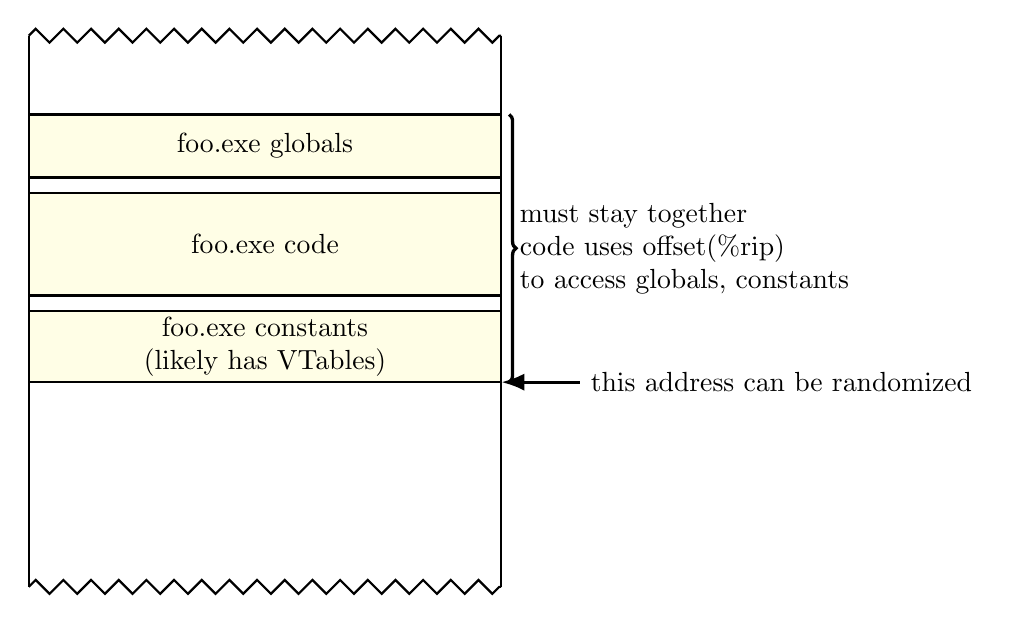
\begin{tikzpicture}[remember picture]
\draw[thick,decorate,decoration={zigzag}] (0, 0) -- (6, 0);
\draw[thick] (0, 0) -- (0, -7);
\draw[thick] (6, 0) -- (6, -7);
\draw[thick,decorate,decoration={zigzag}] (0, -7) -- (6, -7);
\draw[thick,fill=yellow!10] (0, -1) rectangle ++(6, -0.8) node[midway] {foo.exe globals};
\draw[thick,fill=yellow!10] (0, -2) rectangle ++(6, -1.3) node[midway] {foo.exe code};
\draw[thick,fill=yellow!10] (0, -3.5) rectangle ++(6, -0.9) node[midway,align=center] {foo.exe constants \\ (likely has VTables)};
\draw[very thick,Latex-] (6, -4.4) -- ++ (1cm, 0cm) node[right] {this address can be randomized};
\draw[very thick,decorate,decoration={brace,mirror}] (6.1, -4.4) -- ++ (0cm, 3.4) node[midway,right,align=left] {
    must stay together \\
    code uses offset(\%rip) \\
    to access globals, constants
};
\end{tikzpicture}
\end{frame}



\begin{frame}[fragile,label=betweenSegments1]{dependencies between segments (1)}
\begin{lstlisting}[language={},style=smaller]
$ objdump -x foo.exe
...
LOAD off    0x0000000000000000 vaddr 0x0000000000000000 paddr 0x0000000000000000 align 2**12
     filesz 0x0000000000000620 memsz 0x0000000000000620 flags r--
LOAD off    0x0000000000001000 vaddr 0x0000000000001000 paddr 0x0000000000001000 align 2**12
     filesz 0x0000000000000205 memsz 0x0000000000000205 flags r-x
LOAD off    0x0000000000002000 vaddr 0x0000000000002000 paddr 0x0000000000002000 align 2**12
     filesz 0x0000000000000150 memsz 0x0000000000000150 flags r--
LOAD off    0x0000000000002db8 vaddr 0x0000000000003db8 paddr 0x0000000000003db8 align 2**12
     filesz 0x000000000000025c memsz 0x0000000000000260 flags rw-
\end{lstlisting}
\begin{itemize}
\item 4 seperately loaded segments: can we choose random addresses for each?
\end{itemize}
\end{frame}

\begin{frame}[fragile,label=betweenSegments2]{dependencies between segments (2)}
\begin{lstlisting}[language={},style=smaller,moredelim={**[is][\btHL<1->]{~2~}{~end~}}]
0000000000001050 <__printf_chk@plt>:
    1050:       f3 0f 1e fa             endbr64 
    1054:       f2 ff 25 75 2f 00 00    bnd jmpq *~2~0x2f75(%rip)        # 3fd0~end~ <__printf_chk@GLIBC_2.3.4>
    105b:       0f 1f 44 00 00          nopl   0x0(%rax,%rax,1)
\end{lstlisting}
\begin{itemize}
\item dependency from 2nd LOAD (0x1000-0x1205) to 4th LOAD (0x3db8-0x4018)
\item uses relative addressing rather than linker filling in address
\end{itemize}
\end{frame}

\begin{frame}[fragile,label=betweenSegments3]{dependencies between segments (3)}
\begin{lstlisting}[language={},style=smaller,moredelim={**[is][\btHL<1->]{~2~}{~end~}}]
0000000000001060 <main>:
    1060:       f3 0f 1e fa             endbr64 
    1064:       50                      push   %rax
    1065:       8b 15 a5 2f 00 00       mov    0x2fa5(%rip),%edx        # 4010 <global>
    106b:       48 8d 35 92 0f 00 00    lea    ~2~0xf92(%rip)~end~,%rsi        # 2004 <_IO_stdin_used+0x4>
    1072:       31 c0                   xor    %eax,%eax
    1074:       bf 01 00 00 00          mov    $0x1,%edi
    1079:       e8 d2 ff ff ff          callq  1050 <__printf_chk@plt>
\end{lstlisting}
\begin{itemize}
\item dependency from 2nd LOAD (0x1000-0x1205) to 3rd LOAD (0x2000-0x2150)
\item uses relative addressing rather than linker filling in address
\end{itemize}
\end{frame}

\begin{frame}[fragile,label=whyRipRelative]{why is this done?}
\begin{itemize}
\item Linux made a choice: \\
no editing code when loading programs, libraries\
\vspace{.5cm}
\item allows same code to be loaded in multiple processes
\end{itemize}
\end{frame}

\begin{frame}[fragile,label=noGuessing]{danger of leaking pointers}
    \begin{itemize}
        \item any stack pointer? know everything on the stack!
        \item any pointer within executable? know everything in the executable!
        \item any pointer to a particular library? know everything in library!
    \end{itemize}
\end{frame}


\subsection{exercise: using a leak}
\begin{frame}[fragile,label=useLeak1]{exericse: using a leak (1)}
\begin{lstlisting}[language=C++,style=small]
class Foo {
    virtual const char *bar() { ... }
};
...
Foo *f = new Foo;
printf("%s\n", f);
\end{lstlisting}
\begin{itemize}
\item Part 1: What address is most likely leaked by the above?
    \begin{itemize}
    \item A. the location of the Foo object allocated on the heap
    \item B. the location of the first entry in Foo's VTable"
    \item C. the location of the first instruction of Foo::Foo() (Foo's compiler-generated constructor)"
    \item D. the location of the stack pointer
    \end{itemize}
\end{itemize}
\end{frame}


\begin{frame}[fragile,label=useLeak2]{exercise: using a leak (2)}
\begin{lstlisting}[language=C++,style=script]
class Foo {
    virtual const char *bar() { ... }
};
...
Foo *f = new Foo;
char *p = new char[1024];
printf("%s\n", f);
\end{lstlisting}
\begin{itemize}
\item if leaked value was 0x822003 and in a debugger (with \textbf{different randomization}):
    \begin{itemize}
    \item stack pointer was 0x7ffff000
    \item Foo::bar's address was 0x400000
    \item f's address was 0x900000
    \item f's Vtable's address was 0x403000
    \item a ``gadget'' address from the main executable was 0x401034
    \item a ``gadget'' address from the C library was 0x2aaaa40034
    \item p's address was 0x901000
    \end{itemize}
\item which of the above can I compute based on the leak?
\end{itemize}
\end{frame}


\subsection{exercise: using a leak (2)}
\begin{frame}[fragile]{ex: using information leak (2)}
\begin{Verbatim}[fontsize=\fontsize{9}{10}]
printf("buffer = %p", buffer)
\end{Verbatim}
--- \\
{\small \texttt{buffer = 0x646d06d15040}} \\
--- \\
\begin{Verbatim}[fontsize=\fontsize{9}{10}]
$ objdump -tR a.out
...
0000000000004040 g     O .bss   0000000000000400              buffer
...
0000000000003fb0 R_X86_64_JUMP_SLOT  strlen@GLIBC_2.2.5
$ objdump -d a.out
...
0000000000001090 <strlen@plt>:
    1090:       f3 0f 1e fa             endbr64
    1094:       ff 25 16 2f 00 00       jmp    *0x2f16(%rip)        # 3fb0 <strlen@GLIBC_2.2.5>
    109a:       66 0f 1f 44 00 00       nopw   0x0(%rax,%rax,1)
...
\end{Verbatim}
\begin{itemize}
\item exercise: address to overwrite to make strlen(X) run other code?
\end{itemize}
\end{frame}

\begin{frame}{ex: using information leak (2) soln}
\begin{itemize}
\item buffer address = 0x646d06d15040 - offset = 0x4040  
    \begin{itemize}
    \item printed out actual value
    \end{itemize}
\item offset = 0x646d06d11000
\item GOT entry address = 0x3fb0 + offset = 0x646d06d14fb0
    \begin{itemize}
    \item 0x3fb0 = jump slot location
    \end{itemize}
\end{itemize}
\end{frame}


\section{ASLR cost/history}
\begin{frame}{why not always ASLR?}
    \begin{itemize}
    \item ASLR seems like no-brainer
        \begin{itemize}
        \item have to choose address anyway
        \item why not choose at random?
        \end{itemize}
    \item big problem: performance/code size impacts
    \item (smaller problem: inconsistent behavior when bugs)
    \end{itemize}
\end{frame}

\subsection{Unix PIC history}
\begin{frame}{position-independent code}
    \begin{itemize}
    \item position-independent code = code that can be loaded anywhere
        \begin{itemize}
        \item no hard-coded addresses
        \end{itemize}
    \item necessary prerequisite for most of ASLR
    \vspace{.5cm}
    \item Unix did this for libraries for non-security reasons
        \begin{itemize}
        \item share memory between multiple programs loading same library
        \item allow programs to load libraries at any location
        \end{itemize}
    \item but not other programs, probably because of overheads
    \end{itemize}
\end{frame}


\subsection{alternate approach: Windows}

\begin{frame}{relocating: Windows}
    \begin{itemize}
        \item Windows will \myemph{edit code} to relocate
            \begin{itemize}
            \item not everything uses a GOT-like lookup table
            \end{itemize}
        \item typically one fixed location per program/library \textbf{per boot}
            \begin{itemize}
                \item same address used across all instances of program/library
                \item still allows sharing memory
            \end{itemize}
        \item fixup once per program/library per boot
            \begin{itemize}
                \item before ASLR: code could be pre-relocated
            \end{itemize}
        \item Windows + Visual Studio had `full' ASLR by default since 2010
    \end{itemize}
\end{frame}

\begin{frame}{Windows ASLR limitation}
    \begin{itemize}
        \item same address in all programs --- not very useful against local exploits
    \end{itemize}
\end{frame}



\subsection{exercise: without absolute addresses?}
\begin{frame}[fragile,label=ex]{exercise: avoiding absolute addresses}
\lstset{
    language=myasm,
    style=smaller,
    escapeinside=~~,
}
\begin{tikzpicture}
\node[anchor=north east] (code) at (-1, 0) {
\begin{lstlisting}
foo:
	movl	$3, %eax
	cmpq	$5, %rdi
	ja	defaultCase
	jmp	*lookupTable(,%rdi,8)
returnOne:
        movl    $1, %eax
        ret
returnTwo:
        movl    $2, %eax
defaultCase:
        ret
\end{lstlisting}
};
\node[anchor=north west] (code2) at (-.5, 0) {
\begin{lstlisting}
lookupTable:
    .quad returnOne
    .quad returnTwo
    .quad returnOne
    .quad returnTwo
    .quad returnOne
    .quad returnOne
\end{lstlisting}
};
\end{tikzpicture}
\begin{itemize}
    \item exercise: rewrite this without absolute addresses
    \item but fast
\end{itemize}
\end{frame}



\subsubsection{changes with position-independent code}


\newcommand{\myemphTwo}[1]{\myemph<2>{#1}}%
\newcommand{\myemphThree}[1]{\myemph<3>{#1}}%
\newcommand{\myemphFour}[1]{\myemph<{#1}}%
\newcommand{\antiEmphThree}[1]{{\color<3>{blue}#1}}%
\newcommand{\antiEmphFour}[1]{{\color<4>{blue}#1}}%
\begin{frame}[fragile,label=PIEjtasm]{PIE jump-table}
\begin{tikzpicture}
\node[anchor=north east] (code) at (-1, 0) {
\lstset{
    language=myasm,
    style=smaller,
    escapeinside=~~,
}
\begin{lstlisting}
foo:
  movl	 $3, %eax
  cmpq	 $5, %rdi
  ja	 retDefault
  leaq	 ~\myemphTwo{jumpTable(\%rip)},~%rax
  movslq ~\myemphTwo{(\%rax,\%rdi,4)},~%rdx
  addq	 %rdx, %rax
  ~\myemphTwo{\bfseries jmp}~   ~\myemphTwo{*\%rax}~
returnTwo:
  movl  $2, %eax
  ret
returnOne:
  movl  $1, %eax
defaultCase:
  ret
\end{lstlisting}
};
\node[anchor=north west] (code2) at ([xshift=2cm]code.north east) {
\lstset{
    language={},
    style=smaller,
    escapeinside=~~,
}
\begin{lstlisting}
  .section	.rodata
jumpTable:
  .long	returnOne-jumpTable
  .long	returnTwo-jumpTable
  .long	returnOne-jumpTable
  .long	returnTwo-jumpTable
  .long	returnOne-jumpTable
  .long	returnOne-jumpTable
\end{lstlisting}
};
\end{tikzpicture}
\end{frame}

\begin{frame}[fragile,label=PIEjt]{PIE jump-table}
\begin{tikzpicture}
\node[anchor=north east] (code) at (-1, 0) {
\lstset{
    language=myasm,
    style=smaller,
    escapeinside=~~,
}
\begin{lstlisting}
~\myemphTwo{00000000000007ab}~ <foo>:
b8 03 00 00 00       	mov    $0x3,%eax
48 83 ff 05             cmp    $0x5,%rdi
77 1b                	ja     7d0 <foo+0x25>
48 8d 05 ab 00 00 00 	lea    ~\myemphThree{0xab(\%rip),}~%rax        # 868
48 63 14 b8          	movslq ~\myemphThree{(\%rax,\%rdi,4),}~%rdx
48 01 d0             	add    %rdx,%rax
ff e0                	jmpq   *%rax
b8 02 00 00 00       	mov    $0x2,%eax
c3                   	retq   
b8 01 00 00 00       	mov    $0x1,%eax
c3                	retq
...
~\textit{\myemphThree{@ 868}}:~ -156 /* offset */
~\textit{\myemphThree{@ 870}}:~ -162
...
\end{lstlisting}
};
\end{tikzpicture}
\end{frame}

\begin{frame}{added cost}
\begin{itemize}
    \item replace \texttt{jmp *jumpTable(,\%rdi,8)}
    \vspace{.5cm}
    \item with:
        \item \texttt{lea} (get table address --- with relative offset)
        \item \texttt{movslq} (do table lookup of offset)
        \item \texttt{add} (add to base)
        \item \texttt{jmp} (to computed base)
\end{itemize}

\end{frame}

\begin{frame}[fragile,label=x86Worse]{32-bit x86 is worse (1)}
    \begin{itemize}
    \item no relative addressing for {\tt mov}, {\tt lea}, \ldots
    \item even changes ``stubs'' for printf:
    \end{itemize}
\lstset{
    language=myasm,
    style=smaller,
    escapeinside=~~,
}
\begin{lstlisting}
// BEFORE: (fixed addresses)
08048310 <__printf_chk@plt>:
 8048310: ff 25 ~\myemphTwo{10 a0 04 08}~  jmp    *0x804a010
    /* 0x804a010 == global offset table entry */

// AFTER: (position-independent)
00000490 <__printf_chk@plt>:
 490:	ff a3 10 00 00 00    jmp    *0x10~\myemphThree{(\%ebx)}~
    /* %ebx --- address of global offset table */
    /* needs to be set by caller */
\end{lstlisting}
\end{frame}

\begin{frame}[fragile,label=x86Worse]{32-bit x86 is worse (1)}
    \begin{itemize}
    \item no relative addressing for {\tt mov}, {\tt lea}, \ldots
    \item even changes ``stubs'' for printf:
    \end{itemize}
\lstset{
    language=myasm,
    style=smaller,
    escapeinside=~~,
}
\begin{lstlisting}
// BEFORE: (fixed addresses)
08049040 <puts@plt>:
 8049040:       ff 25 04 c0 04 08       jmp    *0x804c004

// AFTER: (position-independent)
00000490 <puts@plt>:
 490:	ff a3 10 00 00 00    jmp    *0x10~\myemphThree{(\%ebx)}~
    /* %ebx --- address of global offset table */
    /* needs to be set by caller */
\end{lstlisting}
\end{frame}

\begin{frame}[fragile,label=x86Worse2]{32-bit x86 is worse (2)}
    \begin{itemize}
    \item changes to call
    \end{itemize}
\lstset{
    language=myasm,
    style=smaller,
    escapeinside=~~,
}
\begin{lstlisting}
// BEFORE: (fixed addresses)
 8049061:  68 08 a0 04 08      push   $0x804a008
 8049066:  e8 d5 ff ff ff      call   8049040 <puts@plt>

// AFTER: (position-independent)
000010d0 <__x86.get_pc_thunk.bx>:
    10d0:  8b 1c 24            mov    (%esp),%ebx
    10d3:  c3                  ret
...

    106e:  e8 5d 00 00 00      call   10d0 <__x86.get_pc_thunk.bx>
    1073:  81 c3 65 2f 00 00   add    $0x2f65,%ebx
...
    107d:  8d 83 30 e0 ff ff   lea    -0x1fd0(%ebx),%eax
    1083:  50                  push   %eax
    1084:  e8 b7 ff ff ff      call   1040 <puts@plt>
\end{lstlisting}
\end{frame}




\subsubsection{recall: vtable pointers?}
\begin{frame}[fragile,label=relocVTable]{extra relocations}
\begin{lstlisting}[language=C++,style=smaller]
struct Foo {
    virtual const char *bar() { return "Foo::bar"; }
};

int main() {
    Foo *f = new Foo;
    f->bar();
}
\end{lstlisting}
\begin{itemize}
\item needed: VTable for Foo
\item contains function pointers --- but function addresses change
\item how is that setup? extra work on program loading
\end{itemize}
\end{frame}

\begin{frame}[fragile,label=relocVTable2]{position-independent versus not}
\begin{Verbatim}[fontsize=\fontsize{8}{9}\selectfont]
$ objdump -R example2

example2:     file format elf64-x86-64

DYNAMIC RELOCATION RECORDS
OFFSET           TYPE              VALUE 
0000000000003da8 R_X86_64_RELATIVE  *ABS*+0x0000000000001160
0000000000003db0 R_X86_64_RELATIVE  *ABS*+0x0000000000001120
0000000000004008 R_X86_64_RELATIVE  *ABS*+0x0000000000004008
0000000000003fd8 R_X86_64_GLOB_DAT  __cxa_finalize@GLIBC_2.2.5
0000000000003fe0 R_X86_64_GLOB_DAT  _ITM_deregisterTMCloneTable
0000000000003fe8 R_X86_64_GLOB_DAT  __libc_start_main@GLIBC_2.2.5
0000000000003ff0 R_X86_64_GLOB_DAT  __gmon_start__
0000000000003ff8 R_X86_64_GLOB_DAT  _ITM_registerTMCloneTable
0000000000003fd0 R_X86_64_JUMP_SLOT  _Znwm@GLIBCXX_3.4
\end{Veratim}
\hrule
\begin{Verbatim}[fontsize=\fontsize{8}{9}\selectfont]
$ objdump -R example2-nopie

example2-nopie:     file format elf64-x86-64

DYNAMIC RELOCATION RECORDS
OFFSET           TYPE              VALUE 
0000000000403ff0 R_X86_64_GLOB_DAT  __libc_start_main@GLIBC_2.2.5
0000000000403ff8 R_X86_64_GLOB_DAT  __gmon_start__
0000000000404018 R_X86_64_JUMP_SLOT  _Znwm@GLIBCXX_3.4
\end{Verbatim}
\end{frame}


\subsection{PIE / PIC}

\begin{frame}{GCC/Clang options}
    \begin{itemize}
    \item -fPIC: generate position-independent code for library
        \begin{itemize}
        \item -fpic --- possibly less flexible/faster version on some platforms
        \end{itemize}
    \item -fPIE, -fpie: generate position-independent code for executable
    \item -pie: link position-independent executable
        \begin{itemize}
        \item -no-pie: don't (where -pie is default)
        \end{itemize}
    \item -shared: link shared library
    \end{itemize}
\end{frame}

\begin{frame}[fragile]{-fPIC/-fPIE differences}
\begin{Verbatim}[fontsize=\small]
extern int foo;
int example() {return foo;}
\end{Verbatim}
with -fPIC:
\begin{Verbatim}[fontsize=\small]
0000000000000000 <example>:
   0:   48 8b 05 00 00 00 00    mov    0x0(%rip),%rax        # 7 <example+0x7>
              3: R_X86_64_REX_GOTPCRELX       foo-0x4
   7:   8b 00                   mov    (%rax),%eax
   9:   c3                      ret
\end{Verbatim}
with -fPIE:
\begin{Verbatim}[fontsize=\small]
0000000000000000 <example>: 
   0:   8b 05 00 00 00 00       mov    0x0(%rip),%eax        # 6 <example+0x6>
              2: R_X86_64_PC32        foo-0x4
   6:   c3                      ret
\end{Verbatim}
\end{frame}

\begin{frame}{GOTPCREL}
    \begin{itemize}
    \item saw two different relocations for global \texttt{int foo}:
    \item \texttt{R\_X86\_64\_PC32} relocation = 32-bit offset to variable
        \begin{itemize}
        \item okay in executable: we'll figure out where \texttt{foo} is
        \item will redirect libraries to use exectuable version
        \end{itemize}
    \item \texttt{R\_X86\_64\_REX\_GOTPCRELX} relocation = 32-bit offset to global offset table entry containing address
        \begin{itemize}
        \item \texttt{foo}'s location decided at runtime by linker
        \item runtime linker writes pointer to library's global offset table
        \item (`REX' part says where instruction starts relative to constant, for fancy linkers)
        \end{itemize}
    \end{itemize}
\end{frame}

\begin{frame}{global offset tableS?}
    \begin{itemize}
    \item executable and library loaded at different addresses
    \item each has own global offset table loaded next to it
    \end{itemize}
\end{frame}


\subsection{PIC cost measurements}
\usetikzlibrary{calc}
\begin{frame}{position independence cost (32-bit)}
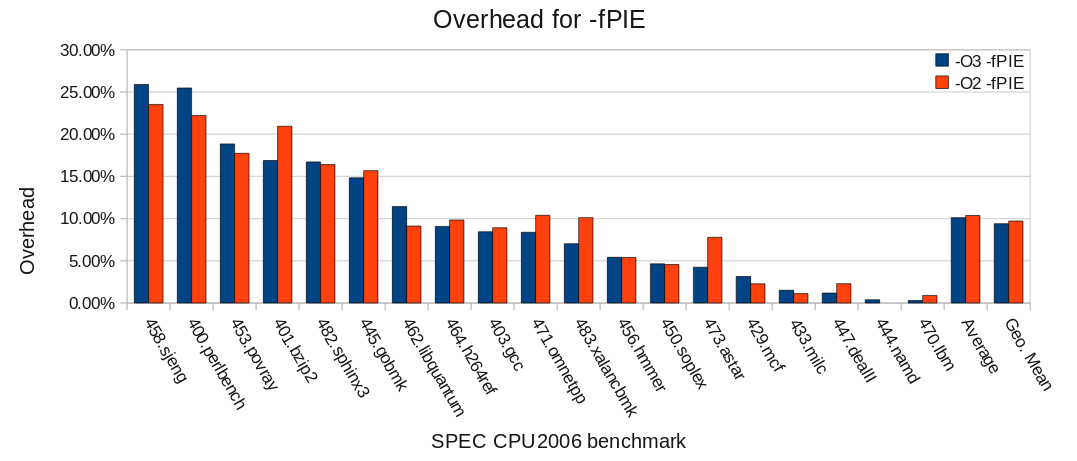
\includegraphics[width=\textwidth]{../mitigate/pie-cost}
\imagecredit{Payer, ``Too much PIE is bad for performance'', ETH Zurich Tech Report}
\end{frame}

\begin{frame}{position independence cost: Linux}
\begin{itemize}
    \item geometric mean of SPECcpu2006 benchmarks on x86 Linux
        \begin{itemize}
            \item with particular version of GCC, etc., etc.
        \end{itemize}
    \item 64-bit: 2-3\% (???)
        \begin{itemize}
        \item ``preliminary result''; couldn't find reliable published data
        \end{itemize}
    \item 32-bit: 9-10\%
    \item depends on compiler, \ldots
\end{itemize}
\end{frame}

\begin{frame}{position independence: deployment}
\begin{itemize}
    \item common for a very long time in dynamic libraries
    \item default for all executables in\ldots
    \vspace{.5cm}
    \item Microsoft Visual Studio 2010 and later
        \begin{itemize}
        \item \texttt{DYNAMICBASE} linker option
        \end{itemize}
    \item OS since 10.7 (2011)
    \item Fedora 23 (2015) and Red Hat Enterprise Linux 8 (2019) and later
        \begin{itemize}
        \item default for ``sensitive'' programs earlier
        \end{itemize}
    \item Ubuntu 16.10 (2016) and later (for 64-bit), 17.10 (2017) and later (for 32-bit)
        \begin{itemize}
        \item default for ``sensitive'' programs earlier
        \end{itemize}
\end{itemize}
\end{frame}


